\section{Background}\label{background}

Human and more than that machine consciousness is called the `Hard
problem' for obvious reasons. The efforts that are
direction are enormous at the moment: Daniel Dennet, David Chalmers,
Marvin Minsky, Aaron Sloman, Antonio Damasio that are most significant
thinkers that work currently in this field. More than that projects like
Blue Brain Project and Human Brain Project declare their goal to impact
the understanding the human consciousness phenomena. The concentration
of funding and computational power is the indication of the highest
interest of modern computer society to the topic of consciousness and
machine consciousness in particular. The complexity of the problem
increases because this field involves several cross-disciplinary
research fields from Cognitive Science (cognitive hexagon):
Neuroscience, Psychology, Philosophy, Anthropology and Sociology. This
puts us in the context of cross disciplinary research of:
neuro-psychology, neuro-philosophy and all of them mapped to
computational systems scientists and engineers.

\section{Objectives}\label{objectives}

The ultimate goal of the project is to create the cognitive architecture
with the option of human consciousness with close to realistic, but
still effective in modern Von Neumann architectures, neurobiological
processes. We have to use some simplification that should be based on
understanding of brain work principles. In other words main goal is to
create cognitive architecture with realistic for modern computers
(clusters) performance implementation of neurobiological nature of
mental processes. We decided to use two cognitive architectures of
Marvin Minsky and Aaron Sloman that provide the complete picture of
human mental processes. Marvin Minsky proposed ``Model of six'' in his
book (Minsky 2007) that contains of six levels of mental activities:

\begin{enumerate}
\def\labelenumi{\arabic{enumi}.}
\itemsep1pt\parskip0pt\parsep0pt
\item
  Instinctive reactions
\item
  Learned reactions
\item
  Deliberative thinking
\item
  Reflective thinking
\item
  Self-reflective thinking
\item
  Self-conscious reflections
\end{enumerate}

With following mechanism of mental processing: Critic -\textgreater{}
Selector -\textgreater{} Way to think / Critic, for details please see
(Minsky 2007).

Aaron Sloman proposed H-CogAff that consist of following parts:

\begin{enumerate}
\def\labelenumi{\arabic{enumi}.}
\item
  Perception mechanisms (hierarchy)
\item
  Actions mechanisms (hierarchy)
\item
  Reactive processes system with alarms
\item
  Deliberative processes system
\item
  Long term associative memory
\item
  Motive activation
\item
  Meta-management (reflective) processes
\item
  Personae
\end{enumerate}

For further details please see (Sloman and Chrisley 2003)

Work breakdown structure is presented below:

\begin{enumerate}
\def\labelenumi{\arabic{enumi}.}
\itemsep1pt\parskip0pt\parsep0pt
\item
  Develop theoretical model of cognitive architecture with option of
  consciousness encapsulating:

  \begin{enumerate}
  \def\labelenumii{\arabic{enumii}.}
  \setcounter{enumii}{1}
  \itemsep1pt\parskip0pt\parsep0pt
  \item
    Philosophical point of view (Model of six (Minsky 2007),
    H-CogAff(Sloman and Chrisley 2003))
  \item
    Neurobiological nature of processes in a brain
  \item
    Psychological phenomena: emotions, learning, self-awareness \ldots{}
  \end{enumerate}
\item
  Implementation of abstract/simplified cognitive architectures of Model
  of Six or/and H-CogAff based on theoretical model

  \begin{enumerate}
  \def\labelenumii{\arabic{enumii}.}
  \setcounter{enumii}{1}
  \itemsep1pt\parskip0pt\parsep0pt
  \item
    Study implementation approaches of cognitive architecture
  \item
    Implement approaches in the way of concept software architecture
  \item
    Implement of simplified cognitive architecture as prototype
    generation 0
  \end{enumerate}
\item
  Implementation of more realistic cognitive architectures of Model of
  Six or/and H-CogAff based on theoretical model

  \begin{enumerate}
  \def\labelenumii{\arabic{enumii}.}
  \setcounter{enumii}{1}
  \itemsep1pt\parskip0pt\parsep0pt
  \item
    Study implementation approaches of cognitive architecture
  \item
    Implement approaches in the way of concept software architecture
  \item
    Implement of simplified cognitive architecture prototype generation
    1
  \end{enumerate}
\item
  Implementation of realistic cognitive architectures of Model of Six
  or/and H-CogAff based on theoretical model

  \begin{enumerate}
  \def\labelenumii{\arabic{enumii}.}
  \setcounter{enumii}{1}
  \itemsep1pt\parskip0pt\parsep0pt
  \item
    Study implementation approaches of cognitive architecture
  \item
    Implement approaches in the way of concept software architecture
  \item
    Implement of simplified cognitive architecture prototype generation
    2
  \end{enumerate}
\end{enumerate}

\section{Relevance}\label{relevance}

The Development in the field of artificial intelligence are stimulated
by the rapid increase of data to be processed which, through
formalization, analysis and synthesis, traditional logico-mathematical
methods are not considered sufficient. Research in the field of fuzzy
logic has received wide support.

The main issue in the evolution of Neurobiologically inspired systems is
to understand how mammals brains work (in particular how rats' brains
function, and as a consequence human brain). The current study due to
its cross-disciplinarity has 2 aspects: Medical: rehabilitation of the
brain after patrimonial damage; Artificial intelligence: to reconstruct
the cortical column in computing systems functions and subsequent
expansion to systems capable of performing basic cognitive functions.
Many scientists in Europe and USA work on Neurobiologically inspired
systems research. Here we can mention Blue Brain and Human Brain
projects. The second project had a budget of 1.4 billion Euros. There is
a program in the USA costing 300 million dollars per year. Under this
program, Von Neumann architecture chips have already been developed,
consuming 10 000 times less energy than other current microprocessors.
Current state of the research field creates options for the creation of
self-learning systems comparable with the human brain. At this point we
must mention IBM company (USA) which has outstanding results in research
in this area. They have developed a technology reproducing1 million
neurons in 1 chip. The relevance of cross-disciplinary research in the
field of AI + Neuroscience can not be underestimated, it is necessary to
take into account the creation of the so called ``dumbbell''
laboratories at Harvard, where scientists were asked to work in one lab
to enhance communications. A major breakthrough in the field of robotic
systems is virtually impossible without controls for autonomous robotic
systems, which has demonstrated its extreme inefficiency and
inflexibility, creating a precedent impossible to build a robotic system
that can survive in real life and social interactions.

\section{Methodology}\label{methodology}

For the purposes of the cross-disciplinary research the group of
international scientists was created that includes: neuro-scientist,
psychologist, philosopher and specialists from AI domain.

In the domain presented above there are several possible directions.
First of all most obvious direct mapping of the psychological and/or
philosophical models in to the computational system this was done in
implementations of several cognitive architectures. But, main
disadvantage of strait mapping leads to miss low level details that
could be crucial for implementation of cognitive architectures with
option of machine consciousness.

The other way could be the creation of uniform theory of complex
phenomena like: emotions, awareness, learning, anticipation or
subjective experience that could run through perspectives:
philosophical, psychological, neurobiological:

\begin{figure}[htbp]
\centering

\includegraphics[width=0.9\textwidth]{layers_binding.png}
\caption{Anthropocentric to computer processes mapping}
\end{figure}

Based on this theory the phenomena could be recreated starting from
lowest level of cellular mechanisms rebuilding all the phenomena in the
other perspectives. This approach demands new holistic and functional
ways to deal with complex problems to maintain overall picture and
functions that implements phenomena of overall picture and have low
level mechanisms taken in account in the same time.

On the other hand the view on recreation of psychological and
philosophical phenomena in a computational system puts us in front of
perspective of definition of new domains in computer science:

\begin{figure}[htbp]
\centering

\includegraphics[width=0.9\textwidth]{p3_model.png}
\caption{P\^{}3 model}
\end{figure}

\section{Ubique method}\label{ubique-method}

It is quite common to use functional decomposition method to deal with
the complex problems, but we see one problem of this approach that are
widely used in modern research. Dealing with low-level details
researches usually loose overall picture high-level goals. In contrast
dealing with only high-level descriptions lead to implementation of
inadequate models in computational systems, that was mentioned above. To
avoid both situations we proposed bidirectional approach that should
take in account both functional decomposition and holistic view on the
complex problem like: `hard problem' of machine consciousness, machine
perception, machine self-awareness, subjective experience. This method
could be described like: \textbf{Imagine 1 neuron -\textgreater{}
cortical column \textasciitilde{} 10 000 neurons -\textgreater{}
Brodmann area (V1) 140 million -\textgreater{} Cortex 19 - 23 billions
-\textgreater{} Whole brain 86 billions (10\textsuperscript{14--10}15
Synapses)} Inside this paradigm we should build first overall model that
could describe neuro-psychological and psychologically-philosophical and
neuro-philosophical phenomena and then with proper understanding we
could implement them in the computational systems.

\section{Results}\label{results}

In two years to produce several prototypes that could help to identify
current problems in implementation of the cognitive architecture with
function of consciousness from high-level (philosophical) and low-level
neurobiological perspectives. The main output should be the prototypes
as software and analysis published in scientific journals and presented
on conferences:

\begin{enumerate}
\def\labelenumi{\arabic{enumi}.}
\itemsep1pt\parskip0pt\parsep0pt
\item
  Theoretical cognitive architecture with the function of consciousness
  prototypes v. 1 and v. 2
\item
  Neuromodulatory cognitive architecture (NEUCOGAR) Dopamine prototype,
  Serotonin prototype and Noradrenaline prototype (integrated prototype
\item
  Cortical column topology prototype of generation v. 1 and v. 2
\end{enumerate}

\subsection{Team}\label{team}

\begin{tabular}{|r|l|}
\hline
\textbf{Role} & \textbf{N} \\ \hline
Project manager & 1 \\ \hline
Lead researcher & 2 \\ \hline
Researchers & 4 \\ \hline
Teamlead & 1 FTE \\ \hline 
Architect & 2 FTE \\ \hline
Developer & 6 FTE \\ \hline
\end{tabular}

\section{References}

Minsky, Marvin. 2007. \emph{The Emotion Machine: Commonsense Thinking,
Artificial Intelligence, and the Future of the Human Mind}. Simon \&
Schuster.

Sloman, Aaron, and Ron Chrisley. 2003. ``Virtual Machines and
Consciousness.'' \emph{Journal of Consciousness Studies}.

\section{Project plan}\label{project-plan}

\begin{figure}[htbp]
\centering
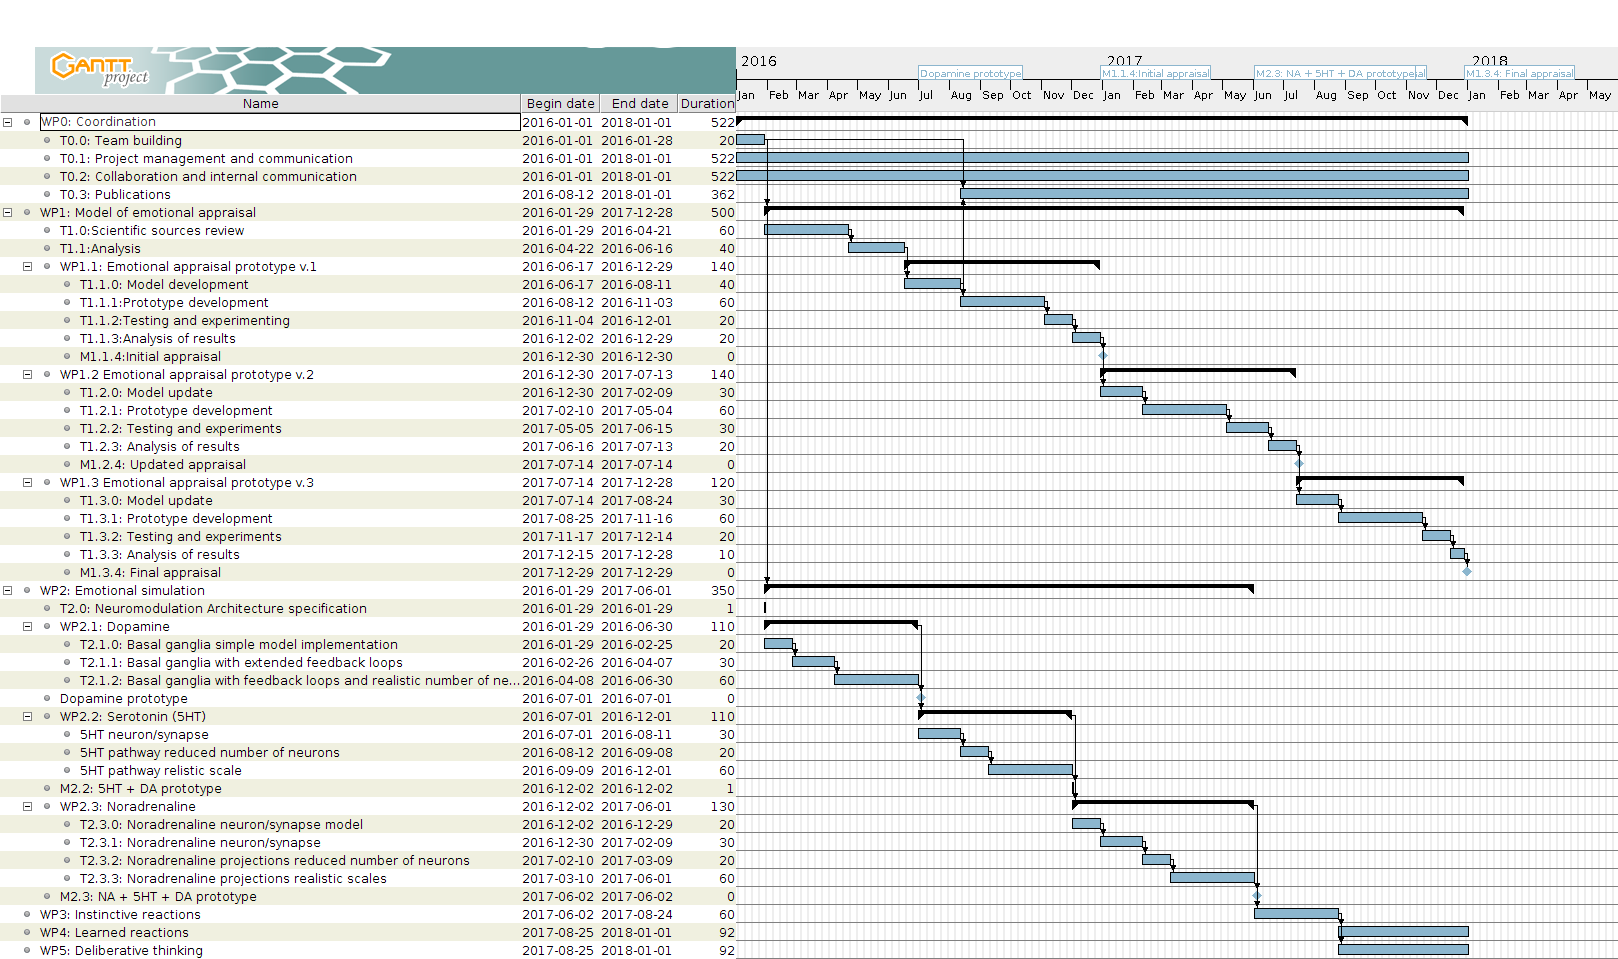
\includegraphics[angle=90, width=1.0\textwidth]{iProject_plan.png}
\caption{AC project plan}
\end{figure}
